\chapter{Odometry}

\section*{Odometry Validation}
The evaluation of the LiDAR odometry and wheel odometry is done by using an overhead camera. To ensure our odometry is accurate enough for use in SLAM, the camera tracks the robot’s movement in real-time and provides a ground-truth odometry reference. Then the data from the camera is compared to the LiDAR and wheel odometry.

The testing procedures were conducted in a monitored environment, using a Logitech C922 PRO HD Stream webcam as the main camera mounted on a studio stand(Figure \ref{fig:camera-setting}). The system was tested on a flat indoor platform without slipperiness or reflection. 

\begin{figure}[H]
    \centering
    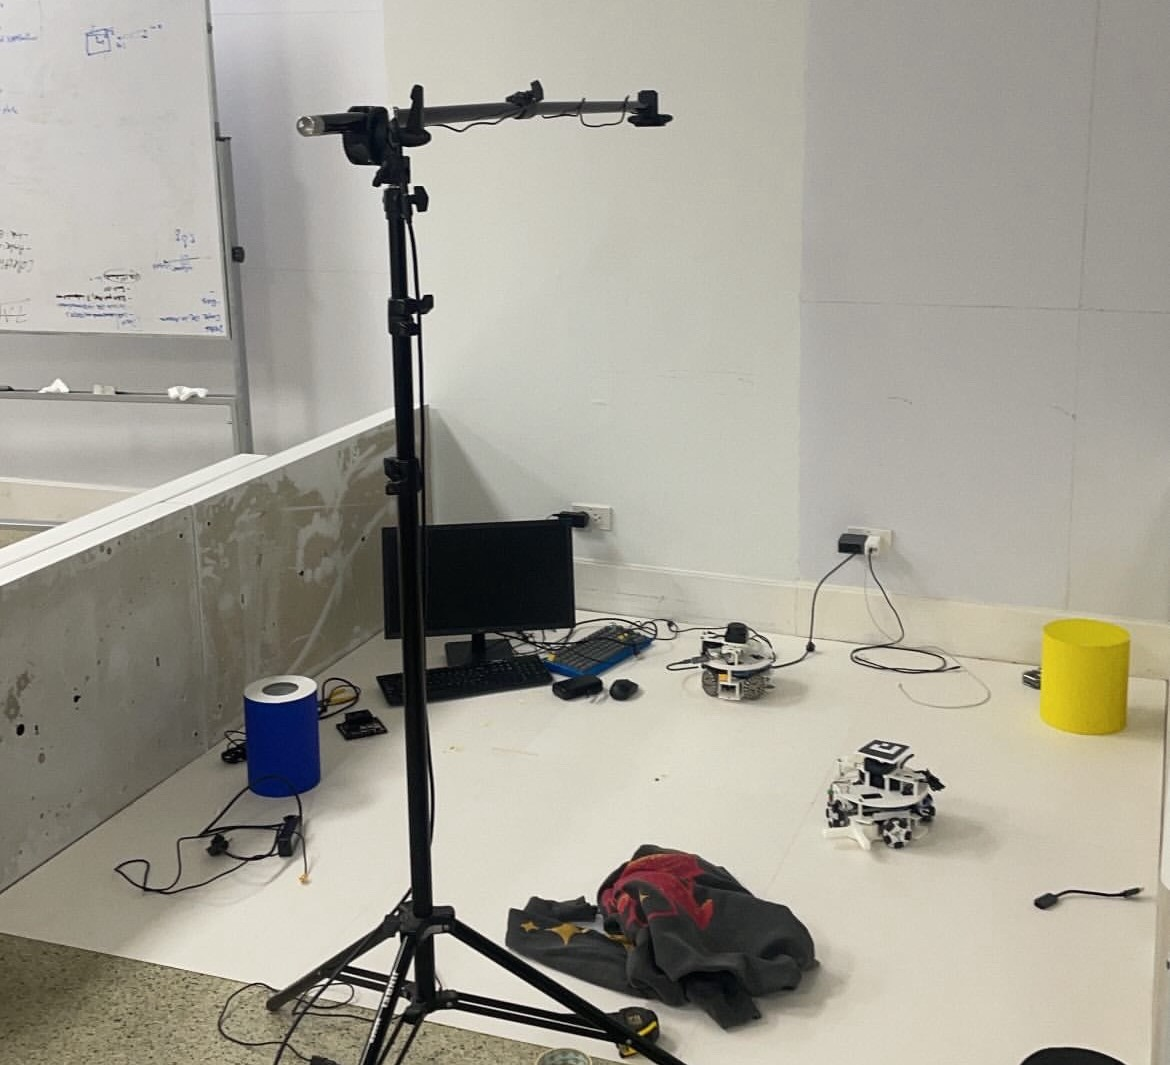
\includegraphics[width=0.3\linewidth]{assets/images/odometry/cam_setting.jpg}
    \caption{Camera Setting}
    \label{fig:camera-setting}
\end{figure}

We use the Augmented Reality University of Cordoba (ArUco) markers to locate the robot's position in the camera frame. DICT\_4×4\_50 ArUco markers were used in the testing because they're the least complex markers, making computation faster and more reliable for real-time detection. After that, the ArUco markers were placed directly above the robot body, while the camera faced directly into the arena.

\begin{figure}[H]
    \centering
    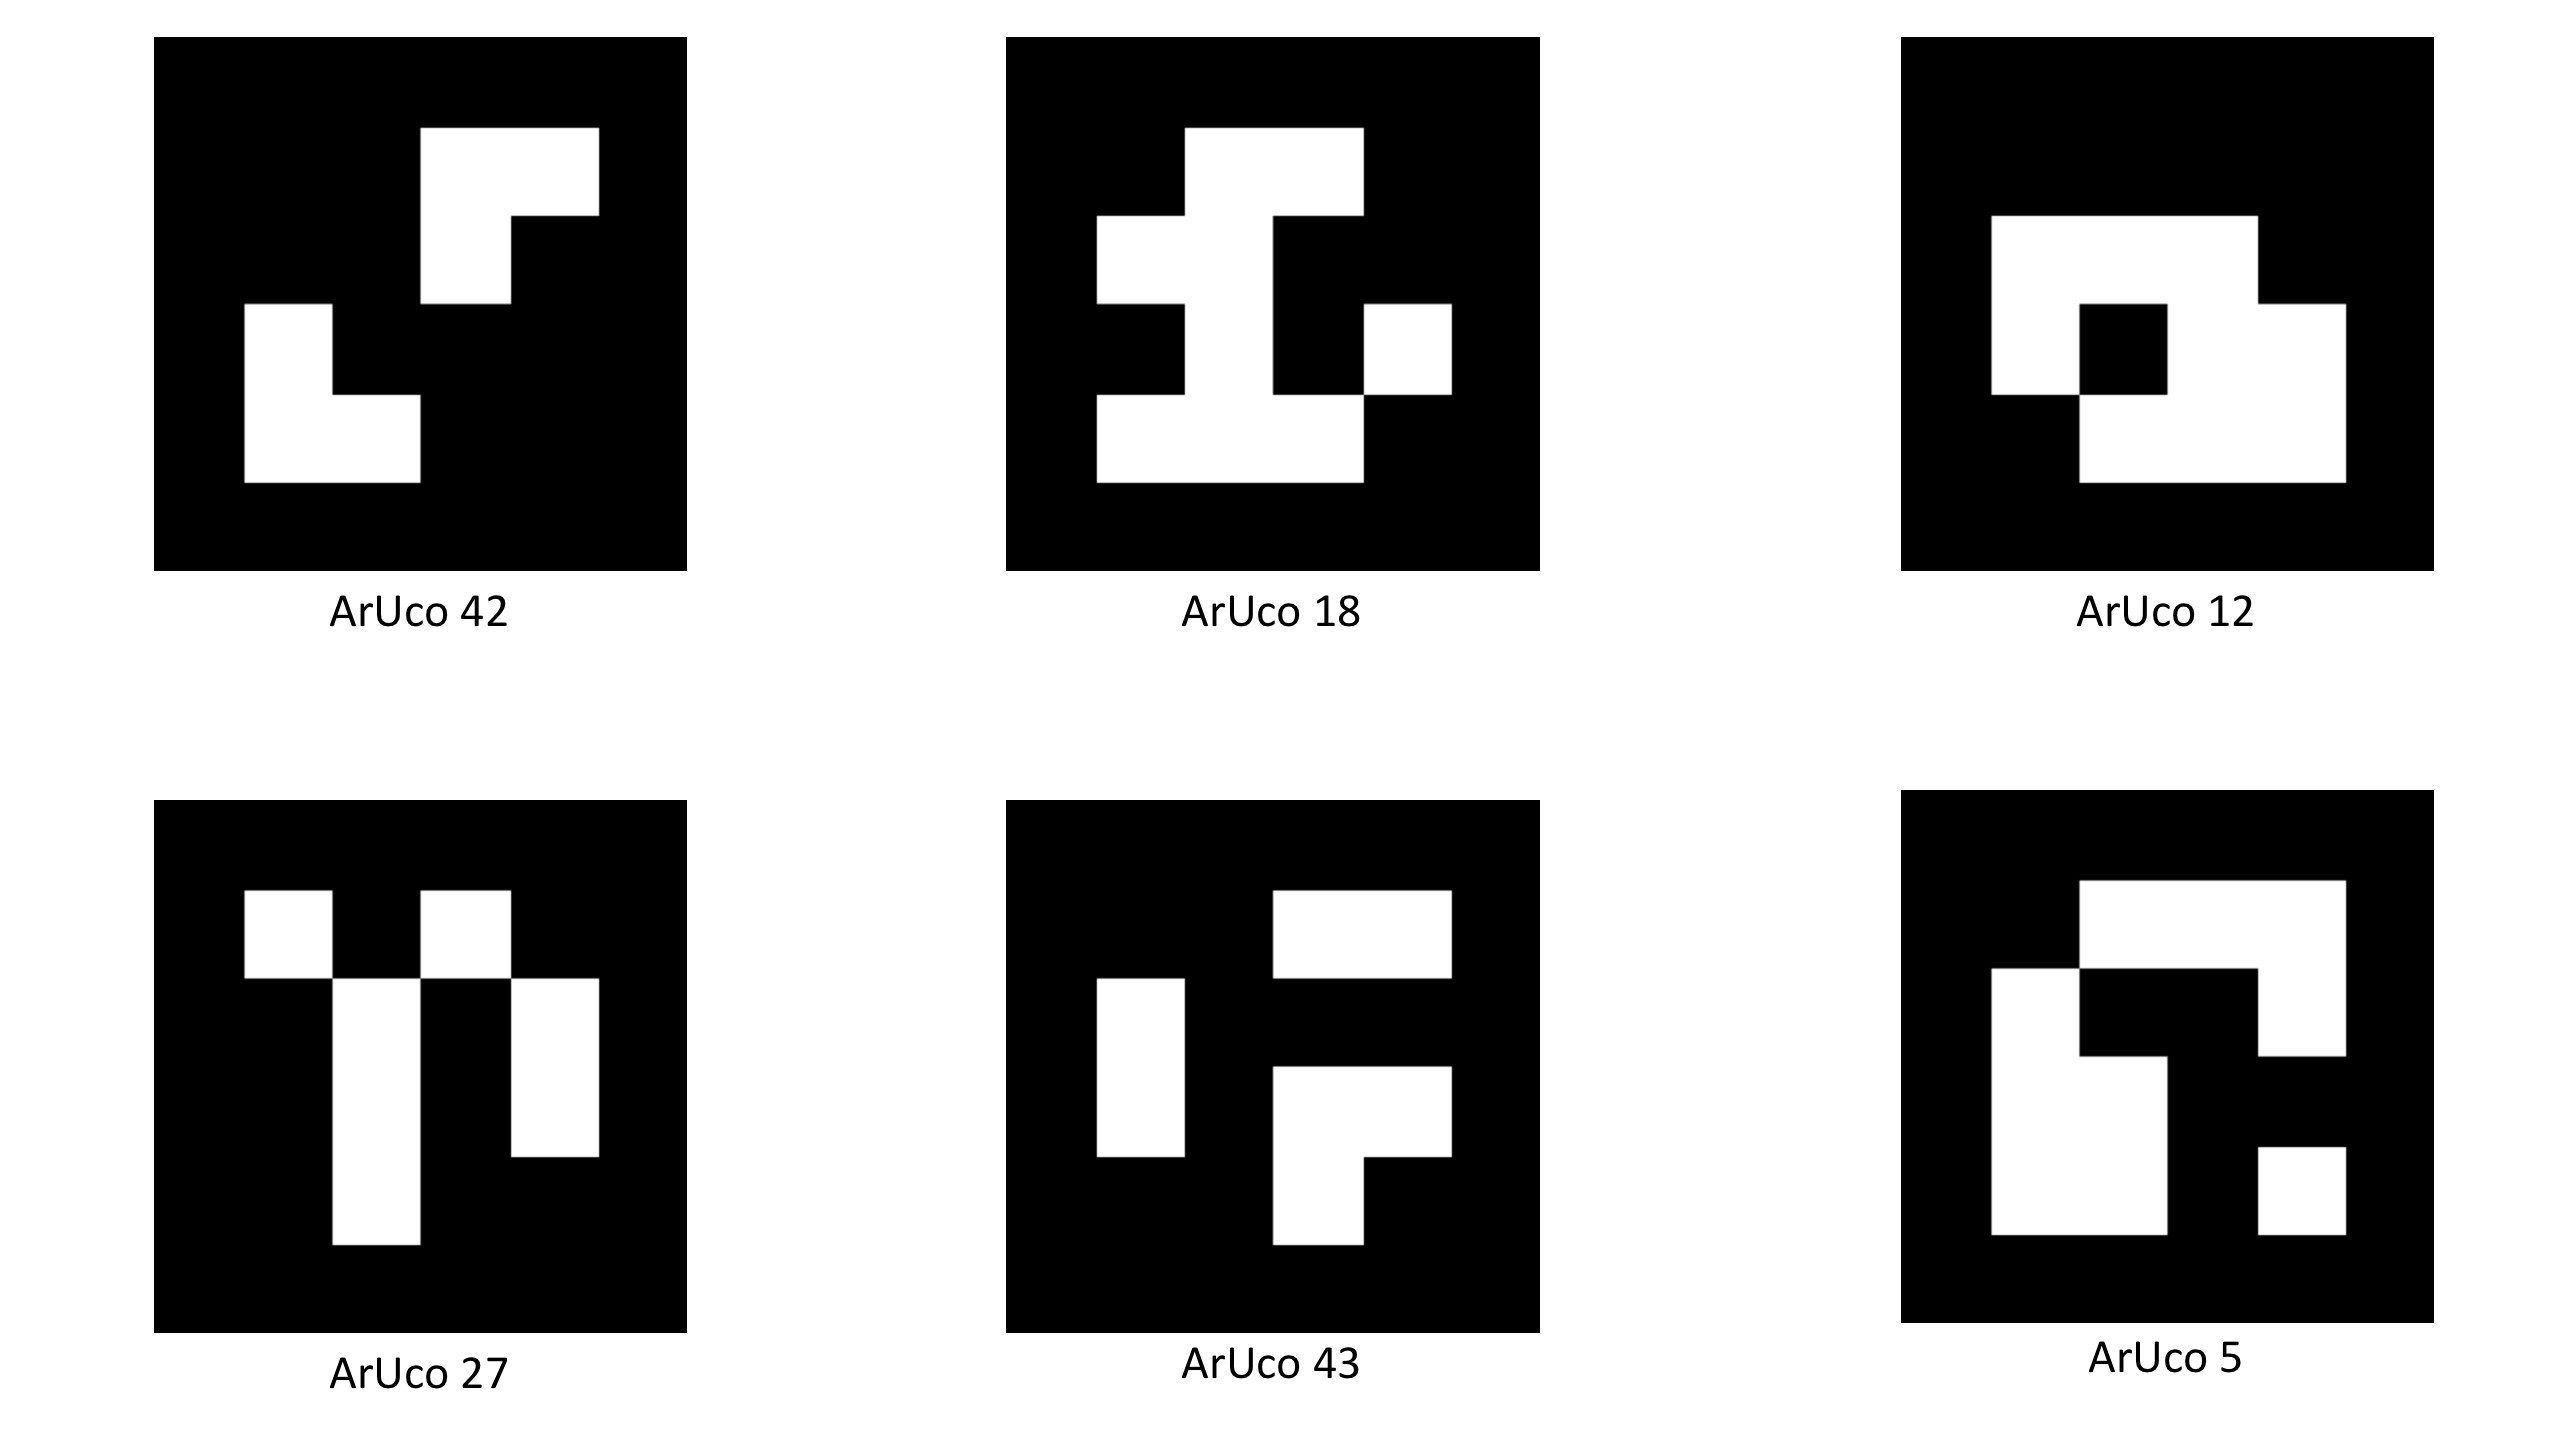
\includegraphics[width=0.4\linewidth]{assets/images/odometry/aruco.png}
    \caption{ArUco markers}
    \label{fig:aruco}
\end{figure}

After that, our overhead camera system extracxted the ArUco's from each frame and calculate the actual position from the map using the Perspective-n-Point (PnP) pose computation.

\subsection*{ArUco Marker Localization}

Given the four detected corner points of an ArUco marker in image coordinates:
\[
\text{Corners} = \{ \mathbf{p}_1, \mathbf{p}_2, \mathbf{p}_3, \mathbf{p}_4 \} = \{ \text{topLeft}, \text{topRight}, \text{bottomRight}, \text{bottomLeft} \}
\]

\paragraph*{1. Center of the Marker}
\[
c_x = \frac{x_{\text{topLeft}} + x_{\text{bottomRight}}}{2}, \quad
c_y = \frac{y_{\text{topLeft}} + y_{\text{bottomRight}}}{2}
\]

\paragraph*{2. Direction Vector of the Top Edge}
\[
\Delta x = x_{\text{topRight}} - x_{\text{topLeft}}, \quad
\Delta y = y_{\text{topRight}} - y_{\text{topLeft}}
\]

\paragraph*{3. Orientation Estimation}
Display orientation in degrees:
\[
\theta_{\text{display}} = \arctan2(\Delta y, -\Delta x)
\]

\paragraph*{4. Normalized Image Coordinates}
Assuming image width $W$ and height $H$:
\[
x_{\text{norm}} = \frac{c_x}{W}, \quad
y_{\text{norm}} = \frac{c_y}{H}
\]

\paragraph*{5. Real-World Position Mapping}
Given real-world map dimensions $S_x$ and $S_y$:
\[
x_{\text{map}} = (x_{\text{norm}} - 0.5) \cdot S_x, \quad
y_{\text{map}} = -(y_{\text{norm}} - 0.5) \cdot S_y
\]

The given formulation allows the transformation of detected 2D marker positions into real-world coordinates as figure shown:

\begin{figure}[H]
    \centering
    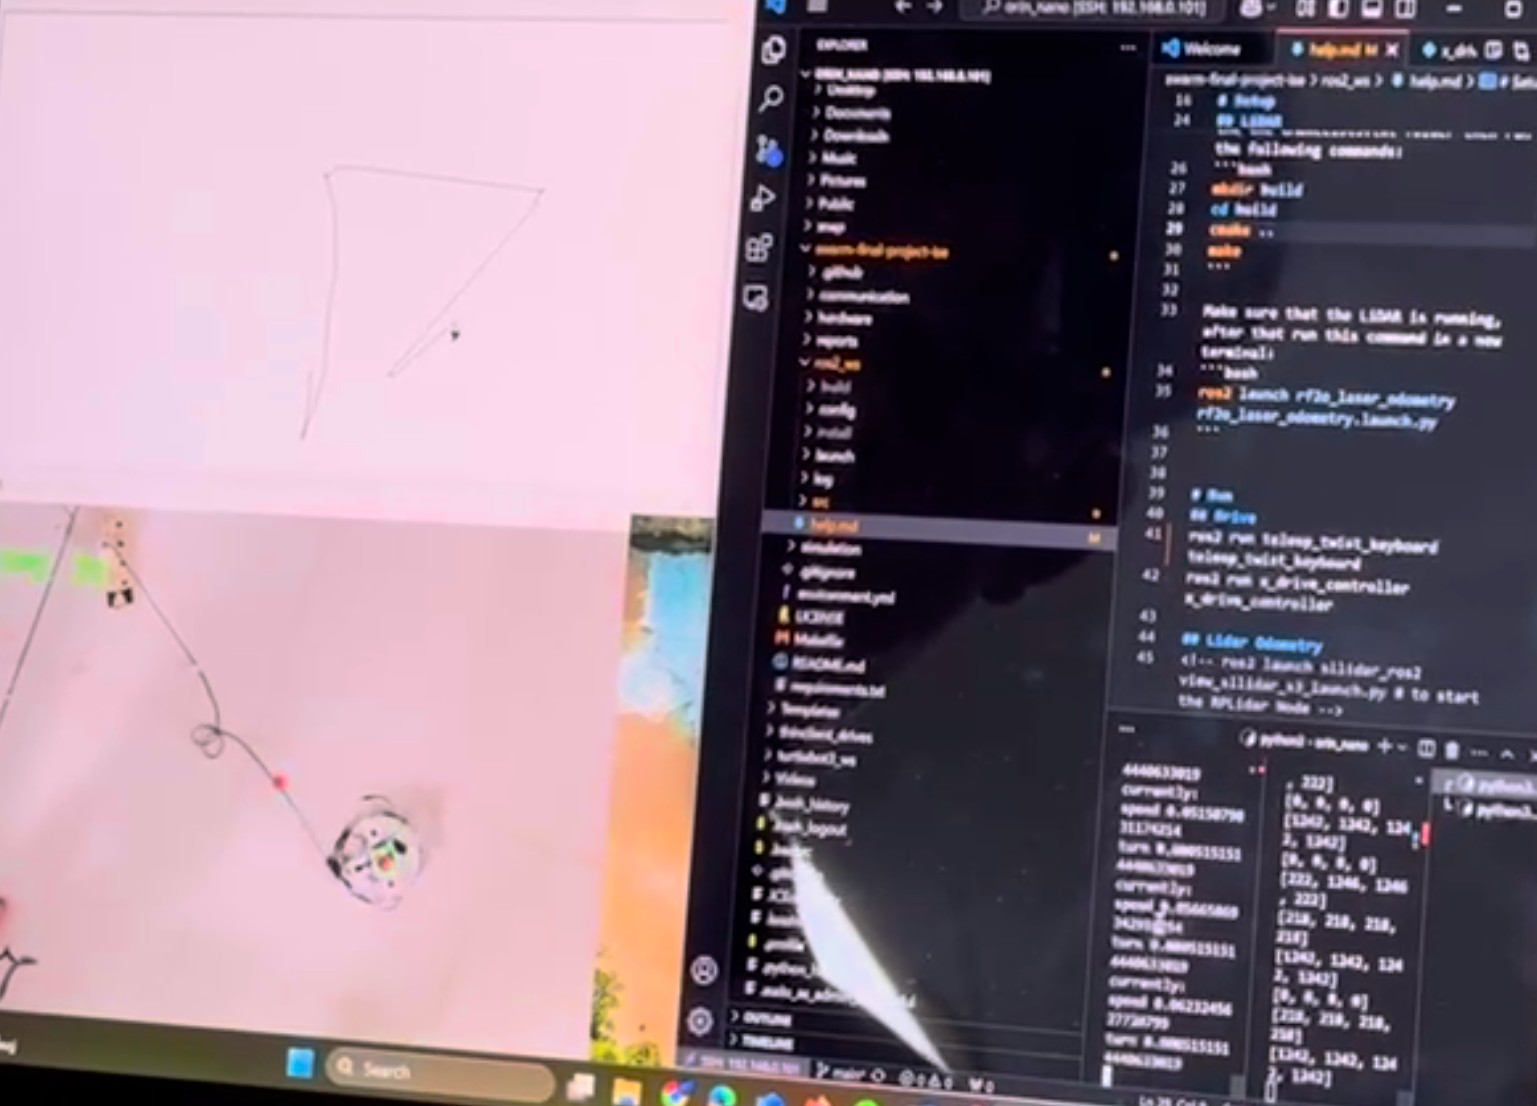
\includegraphics[width=0.6\linewidth]{assets/images/odometry/arena_robot.jpg}
    \caption{Implementing ArUco on the robot}
    \label{fig:aruco-robot}
\end{figure}

After obtaining the data, we then compare the error of the trajectory given from the LiDAR odometry to the actual robot position from the camera. The test included the robot running sideways (holonomic constraint) in a positive x direction for 50 cm, running forward (non-holonomic constraint) in a positive x direction for 50 cm, and turning 360 degrees clockwise and counterclockwise.

\begin{figure}[H]
    \centering
    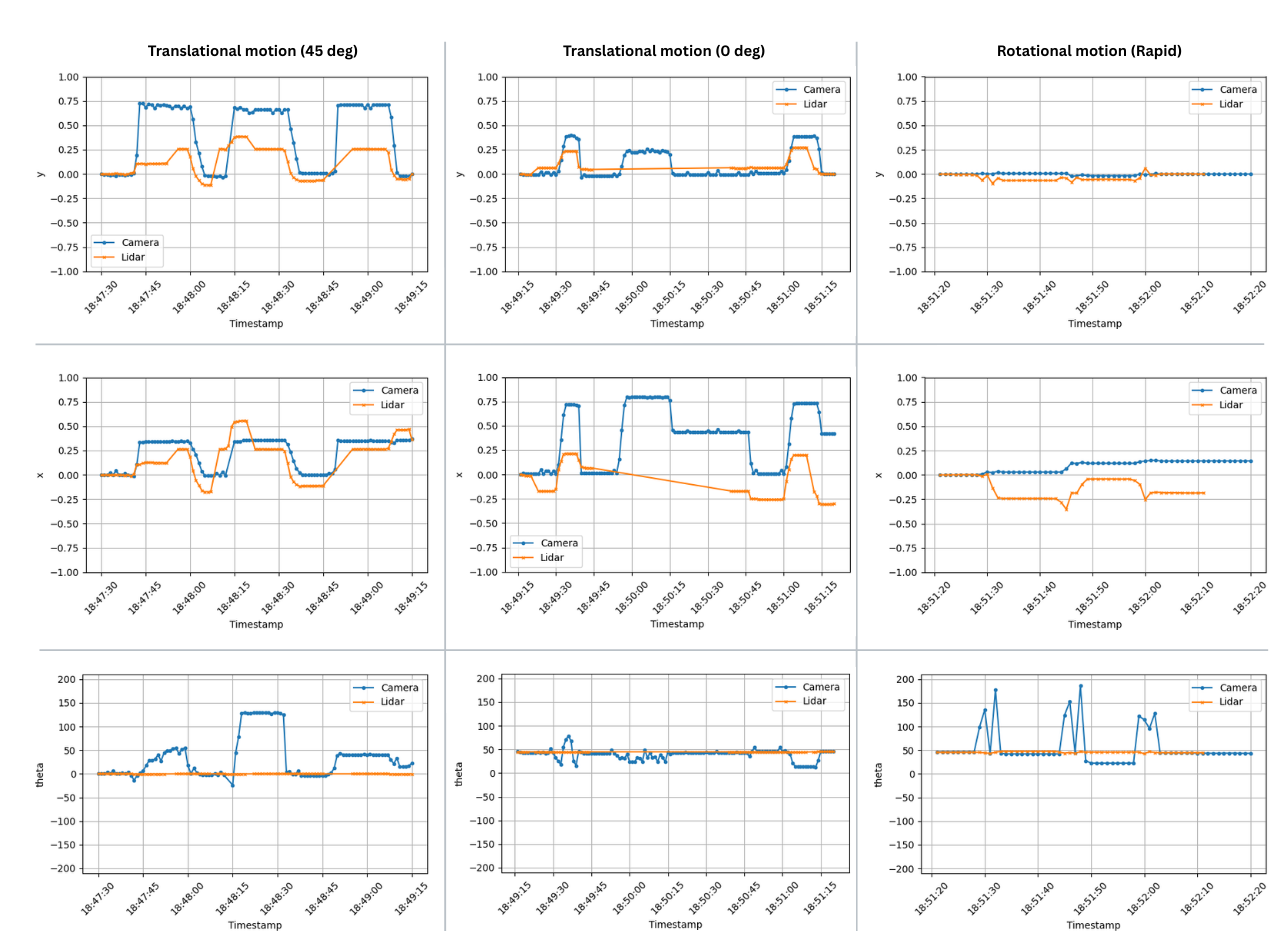
\includegraphics[width=1\linewidth]{assets/images/odometry/detail_visual.png}
    \caption{Result Visualization of LiDAR vs actual odometry}
    \label{fig:detail-result}
\end{figure}

\begin{figure}[H]
    \centering
    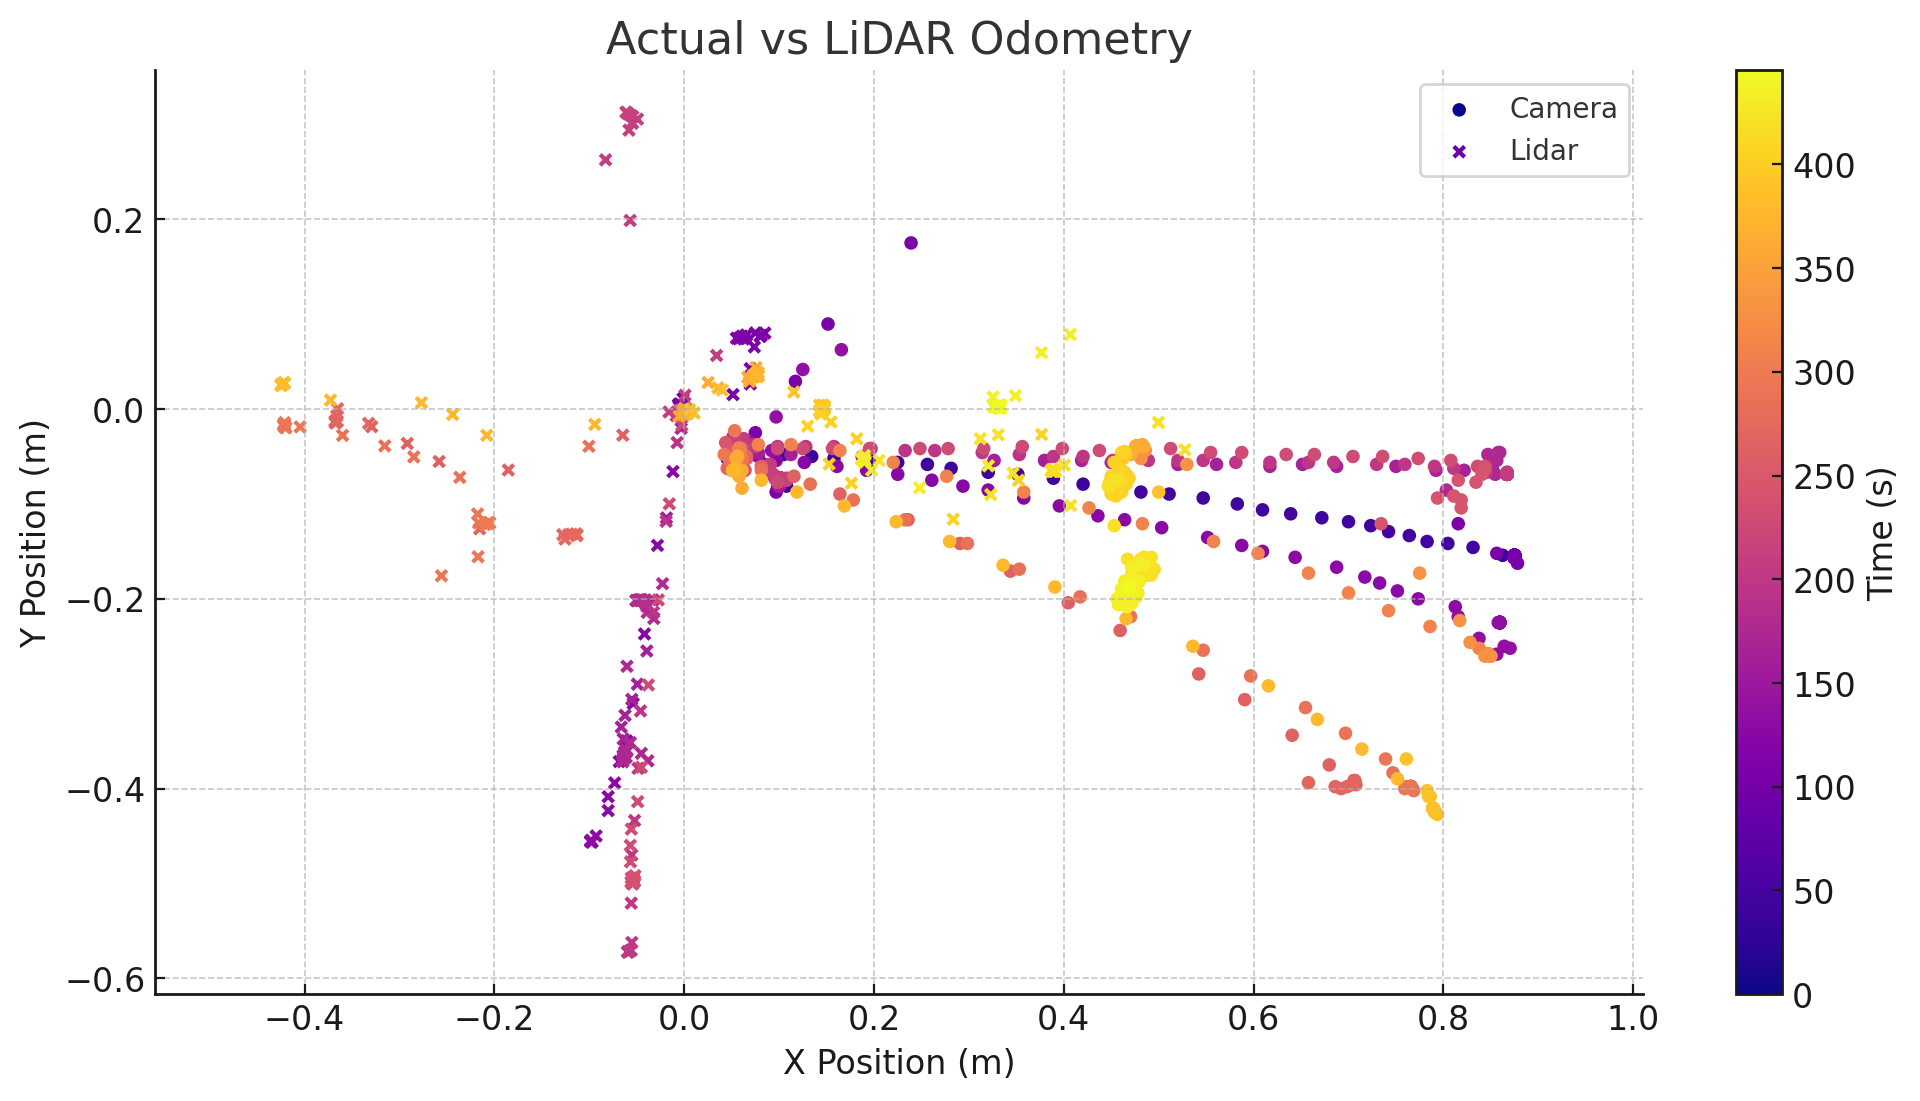
\includegraphics[width=1\linewidth]{assets/images/odometry/testing_visual.png}
    \caption{Result Visualization of LiDAR vs actual odometry in an 2-D plane}
    \label{fig:visual-result}
\end{figure}

From our experiments, we observed that the LiDAR odometry often deviates from the actual trajectory, especially in movements involving rotation or sliding. These discrepancies indicate that the current LiDAR setup may not provide sufficient accuracy for precise localization tasks. As a result, we propose using the overhead camera system with ArUco markers as a temporary but reliable substitute for ground-truth positioning. This approach offers improved consistency and will serve as our main reference until a more robust odometry solution is implemented.
